Ziel dieser Arbeit ist es das Verständnis des simulationstools Simulink zu vertiefen. Dazu soll eine Simulation erstellet werden welche mehrere unterschiedliche physikalische Netzwerke miteinander verbindet. In diesem Bericht wir die Verwendung einer Wasserpumpe aufgezeigt. Dabei bedienen wir uns der Vorlage (sh\_well\_jet\_pump) aus Matlab.\\
\\

%%%%%%%%%%%%%%%%%%%%%%%%%%%%%%%%%%%%%%%%%%%%%%%%%%%%%%%%%%%%%%%%%%%%%%%%%%%%%
\begin{figure}[b]
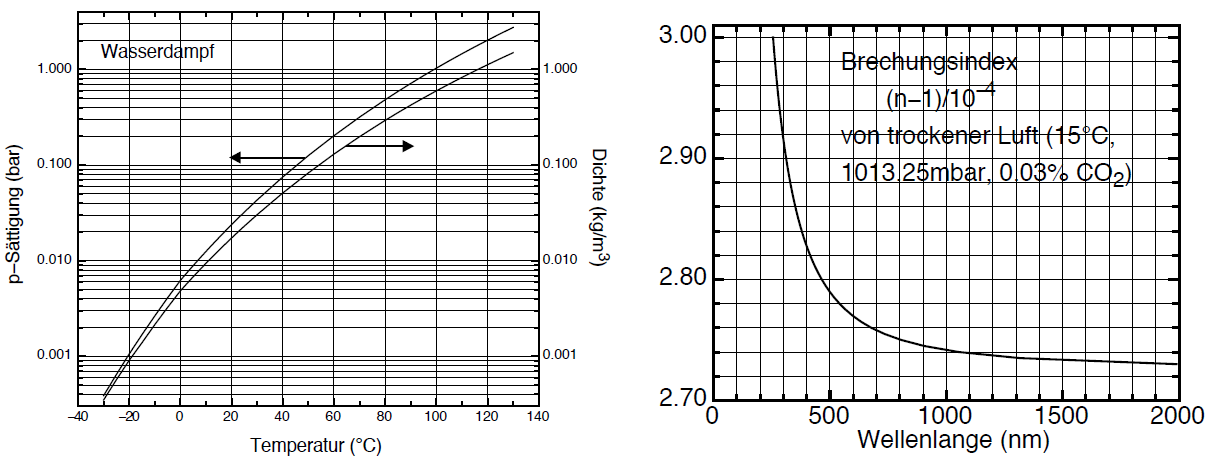
\includegraphics[width=\textwidth]{Brechungsindex_Luft_Grafik.png}
\caption{Wasserdampfsättigung und Normbrechungsindex}
\label{fig:Wasserdampfsättigung und Normbrechungsindex}
\end{figure}
%%%%%%%%%%%%%%%%%%%%%%%%%%%%%%%%%%%%%%%%%%%%%%%%%%%%%%%%%%%%%%%%%%%%%%%%%%%%%
